\documentclass[11pt]{article}

\usepackage{amsmath}
\usepackage{textcomp}
\usepackage[top=0.8in, bottom=0.8in, left=0.8in, right=0.8in]{geometry}
% Add other packages here %
\usepackage{graphicx}
\usepackage{subcaption}
\usepackage{caption}

% Put your group number and names in the author field %
\title{\bf Excercise 3\\ Implementing a deliberative Agent}
\author{Group \textnumero 54: Oriol Barbany Mayor, Natalie Bolón Brun}


% N.B.: The report should not be longer than 3 pages %


\begin{document}
\maketitle

\section{Model Description}

\subsection{Intermediate States}
% Describe the state representation %
We define the current state with the following attributes:
\begin{itemize}
    \item Plan up to the current time
    \item City where the vehicle is currently located
    \item Lists of both tasks to pick and to deliver. When starting a simulation, the list of delivered tasks is empty but if a plan is computed after the cancellation of a plan, the delivery list contains those tasks that the agent already picked. 
    \item Capacity left in the vehicle at current time. When starting a simulation, the capacity is that of the vehicle. 
\end{itemize}

\subsection{Goal State}
% Describe the goal state %
According to the state description specified above, we say that a state is terminal if the list of both the tasks to pick and to deliver are empty.

\subsection{Actions}
% Describe the possible actions/transitions in your model %
For each state, we can go to any of the neighbors of the current city. Moreover, if there are $m$ tasks available in the current city, we consider all subsets of $[m]=\{1,\dots,m\}$ (including the empty set) such that the sum of the capacities of each task do not exceed the capacity that our vehicle still has in the current state. This implies that for each neighbor we have $2^m$ potential new states to explore.

In the case that we can deliver one or more tasks at the current location, we do it, since there is no scenario where not delivering leads to an optimal solution. This latter is because the delivery gives a reward and increases the capacity left in the vehicle.

\section{Implementation}
To implement both algorithms, we define a custom class for each \verb|PlanBuilder| for the A* algorithm and  \verb|PlanBuilderBFS| for BFS. These functions handle the creation and updating of the queue according to the selected algorithm. The queue is implemented as a \verb|PriorityQueue| for A* to speed up the insertion of states in the queue and avoid sorting it. For BFS, it is implemented as \verb|LinkedList| since we do not care about the sorting but rather about fast access to the elements. 

Both planning algorithms are based on a queue that starts with a unique source state. At each iteration, we get the first state in the queue and add all the resulting neighboring states (reachable within one action) to the queue if this neighbor state $s$ has not been visited or it has been but with a larger $f(s)$, which is defined as
\begin{align}
    f(s) := g(s)+ h(s)
\end{align}
where $g(s)$ corresponds to the total distance of the plan of $s$ and $h(s)$ to the value of its heuristic (see section \ref{sec:heu}).

In order to check whether a state was already visited, we store a mapping from hashcodes of the state to its current cost defined as the total distance pursued.

To check the available tasks to pickup (resp. deliver), we create a \verb|HashMap| linking the pickup (resp. delivery) city with the corresponding tasks. Whenever an agent reaches a new city, it only needs to consult the corresponding tasks associated to that city in order to perform the planning. 

\subsection{BFS}
% Details of the BFS implementation %
This algorithm explores all the states that are in the queue and hence terminates when it is empty. During the execution of BFS several goal states are reached, and we store all of them to pick the best one once the algorithm has terminated.

\subsection{A*}
% Details of the A* implementation %
This algorithm explores states until it finds the first goal state. The state explored is always the one with lower associated cost $f(s)$, guiding the exploration towards an optimum. This way, we do not need to explore the whole set of states that we find along the planning to obtain an optimum, thus reducing the time required to compute a plan.

\subsection{Heuristic Function}
\label{sec:heu}
% Details of the heuristic functions: main idea, optimality, admissibility %
The implemented heuristic function associates to each state a future cost given by the total distance of the minimum spanning tree (MST) containing all the cities where there is a task to pickup or deliver. 

The heuristic cost cannot be greater than the real cost of the state. Indeed in a MST we don't have the tasks distributed in such a way that each city only needs to be visited once and also there could be more than two leafs and the current city could not be one of these. Therefore, the MST is a valid lower bound of the true cost.

We find the MST using Kruskal's algorithm and making use of two helper classes. The class \texttt{Edge} define the relation between two cities and each distance. Note that in the original graph (defined by the topology) the vertices of the MST are not necessarily connected. Thus we create a connected graph which edges represent the minimum distance between two cities. Moreover, we also created the class \texttt{Set} as a implementation of the union-find disjoint set structure.

\section{Results}

\subsection{Experiment 1: BFS and A* Comparison}
We compare the performance of the BFS and A* with a single agent in situations with different number of tasks. We aim to evaluate the cost of the final plans and the time required to compute them. 
% Compare the two algorithms in terms of: optimality, efficiency, limitations %
% Report the number of tasks for which you can build a plan in less than one minute %

\subsubsection{Setting}
% Describe the settings of your experiment: topology, task configuration, etc. %
Both agents are evaluated under the same conditions (same starting point, vehicle and task distribution). We use the Swiss topology and the default settings for the probability, rewards and weight of the tasks.

\subsubsection{Observations}
% Describe the experimental results and the conclusions you inferred from these results %
% Please add the following required packages to your document preamble:
\begin{minipage}[]{\textwidth}

\begin{minipage}[]{0.6\textwidth}
\resizebox{\textwidth}{!}{%
\begin{tabular}{|c|c|c|c|c|c|c|c|c|c|c|}
\hline
num. tasks & \multicolumn{2}{c|}{\textbf{6}} & \multicolumn{2}{c|}{\textbf{10}} & \multicolumn{2}{c|}{\textbf{12}} & \multicolumn{2}{c|}{\textbf{15}} & \multicolumn{2}{c|}{\textbf{17}} \\ \hline
algorithm & \textbf{\begin{tabular}[c]{@{}c@{}}cost\\ {[}km{]}\end{tabular}} & \textbf{\begin{tabular}[c]{@{}c@{}}time\\ {[}s{]}\end{tabular}} & \textbf{\begin{tabular}[c]{@{}c@{}}cost\\ {[}km{]}\end{tabular}} & \textbf{\begin{tabular}[c]{@{}c@{}}time\\ {[}s{]}\end{tabular}} & \textbf{\begin{tabular}[c]{@{}c@{}}cost\\ {[}km{]}\end{tabular}} & \textbf{\begin{tabular}[c]{@{}c@{}}time\\ {[}s{]}\end{tabular}} & \textbf{\begin{tabular}[c]{@{}c@{}}cost\\ {[}km{]}\end{tabular}} & \textbf{\begin{tabular}[c]{@{}c@{}}time\\ {[}s{]}\end{tabular}} & \textbf{\begin{tabular}[c]{@{}c@{}}cost\\ {[}km{]}\end{tabular}} & \textbf{\begin{tabular}[c]{@{}c@{}}time\\ {[}s{]}\end{tabular}} \\ \hline
\textbf{BFS} & 1260 & 0 & 1520 & 14 & 1620 & 190 & - & - & - & - \\ \hline
\textbf{A*} & 1260 & 0 & 1520 & 0 & 1620 & 1 & 1810 & 18 & 1810 & 87 \\ \hline
\end{tabular}%
}
\captionof{table}{Time and cost of the final plan computed with BFS or A* for different number of tasks. }
\label{tab:single-agent}
\end{minipage}{}
\hfill
\begin{minipage}[]{0.35\textwidth}
The maximum number of tasks that can be handled to produce a plan under 1 min is 16 for A* (33s) and  11 for BFS. Increasing one task in A* results in an increase of the required time of 54s while for BFS the increase is of 138s (from 52s with 11 tasks to 190s with 12 tasks). 
\end{minipage}{}

\end{minipage}

This points out how much time can be saved using A* without decreasing the quality of the solution in terms of optimality. 

On the other hand, we can see the final cost of the solution remains optimal with A* and stabilizes around a value when we keep increasing the number of tasks. This is due to the topology of our problem which allows to handle multiple tasks at the same time without increasing the km travelled to pickup and deliver these items. 




\subsection{Experiment 2: Multi-agent Experiments}
% Observations in multi-agent experiments %
We perform two different experiments: two agents (one BFS and one A*) and three agents (BFS all).

\subsubsection{Setting}
% Describe the settings of your experiment: topology, task configuration, etc. %
The experiments are done with the Swiss topology, the vehicle's capacity limited to 15kg, the task's weight set to 5kg and with 10 available tasks. We choose this combination of weight and capacity to enforce situations where agents must refuse picking tasks. 

\subsubsection{Observations}
% Describe the experimental results and the conclusions you inferred from these results %

\begin{minipage}[]{\textwidth}

\begin{minipage}[]{0.48\textwidth}
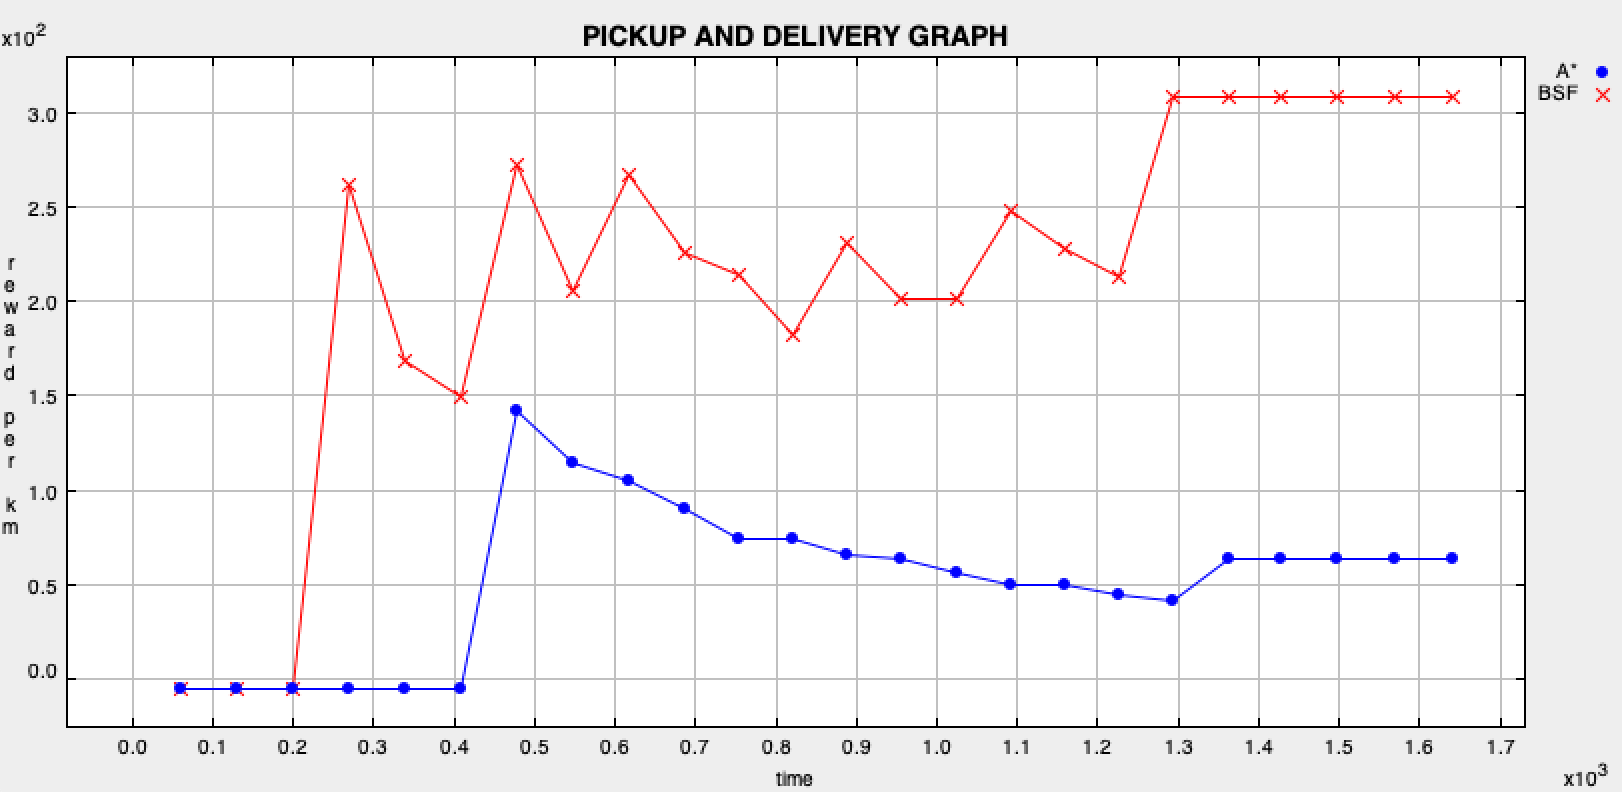
\includegraphics[width=\textwidth]{plots-deliberative/2vehicles.png}
\captionof{figure}{Evolution of reward per km with 2 agents}
\label{fig:2vehicles}

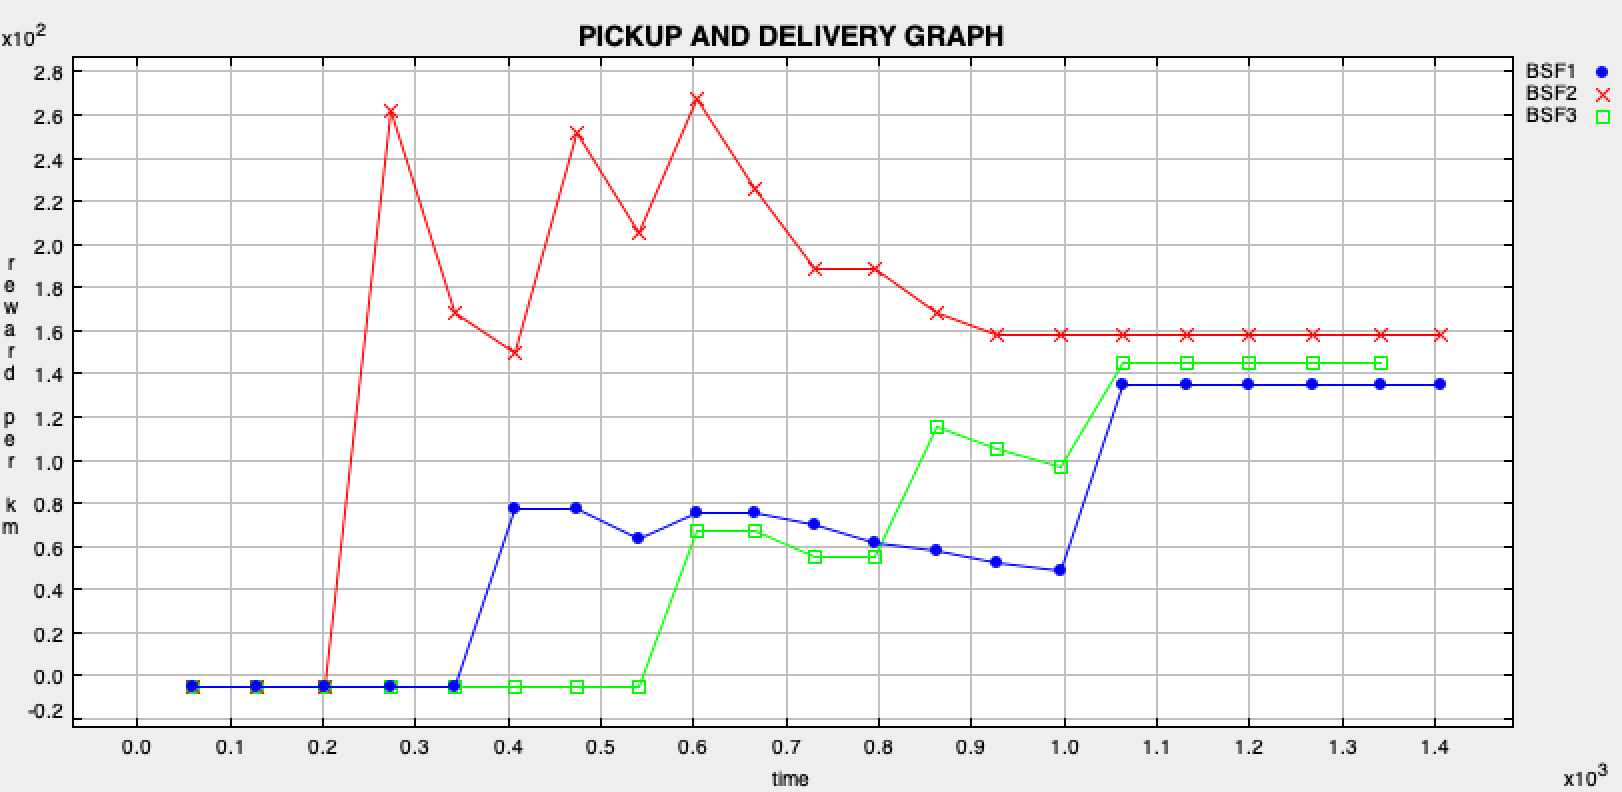
\includegraphics[width=\textwidth]{plots-deliberative/3vehicles.png}
\captionof{figure}{Evolution of reward per km with 3 agents}
\label{fig:3vehicles}
\end{minipage}
\hfill
\begin{minipage}[]{0.5\textwidth}
In the first experiment shown in Figure \ref{fig:2vehicles} we compare two agents. The two agents perform their plans independently, only sharing the information about the available tasks. This results in some unnecessary movements of agents moving towards a point where there is no more an available task. Whenever a plan is cancelled, there is a new plan recomputed which takes into account the current tasks being carried by the agent. We can observe that agent A* makes several movements towards tasks that are already unavailable, resulting in a high cost without reward. 

Figure \ref{fig:3vehicles} shows the performance when working with 3 agents. In this case we have two agents following the same path and alternating the pickups, resulting in a very similar final reward per km. Whenever agent 2 or 3 recompute their plans, the new plan still follows a very similar path to the one of the cancelled plan, what generates this alternation in picking up tasks between the agents. 


\end{minipage}

\end{minipage}

\end{document}